\documentclass[12pt]{article}

% Computational Physics by M. Newman
% Setup file for exercises

% Packages
\usepackage{mathpazo}
\usepackage{amsmath}
\usepackage{graphicx}
\usepackage{calrsfs}
\usepackage{fancyvrb}

% Formatting
\setlength{\textwidth}{17.5cm}
\setlength{\textheight}{24.0cm}
\setlength{\evensidemargin}{2.5cm}
\setlength{\oddsidemargin}{-0.6cm}
\setlength{\topmargin}{-2.3cm}
\setlength{\textfloatsep}{0pt}
\setcounter{secnumdepth}{0}
\renewcommand{\baselinestretch}{1.06}

% Macros
\newcommand{\dd}{\mathrm{d}}
\newcommand{\ii}{\mathrm{i}}
\newcommand{\e}{\mathrm{e}}
\newcommand{\half}{\tfrac12}
\newcommand{\av}[1]{\langle#1\rangle}
\newcommand{\var}{\mathop\mathrm{var}}
\newcommand{\Ord}{\mathrm{O}}
\renewcommand{\Re}{\mathop\mathrm{Re}\nolimits}
\renewcommand{\Im}{\mathop\mathrm{Im}\nolimits}
\newcommand{\mat}{\mathbf}
\renewcommand{\vec}{\mathbf}
\newcommand{\defn}{\textit}
\newcommand{\exskip}{\nopagebreak\medskip\noindent}
\newcommand{\pmstrut}{\rule{0pt}{13pt}}

% Environments
\newcounter{chapter}
\setcounter{chapter}{2}
\newcounter{exercise}
\renewcommand{\theexercise}{\arabic{chapter}.\arabic{exercise}}
\newenvironment{exercises}{\vspace{2ex plus0.5ex minus0.5ex}
  \renewcommand{\labelenumi}{\alph{enumi})}}%
    {\par\vspace{1ex plus0.5ex minus0.5ex}}
\newcommand{\exercise}{\refstepcounter{exercise}%
  \par\vspace{4ex plus1ex minus1ex}%
  \noindent\textbf{Exercise \theexercise: }}

\DefineVerbatimEnvironment{code}{Verbatim}{xleftmargin=\parindent}

\setcounter{chapter}{5}

\begin{document}

\noindent {\LARGE\textsc{Computational Physics}}\par
\bigskip
\noindent {\large\textsc{Exercises for Chapter \arabic{chapter}}}\par
\noindent\hrulefill

%%%%%%%%%%%%%%%%%%%%%%%%%%%%%%%%%%%%%%%%%%%%%%%%%%%%%%%%%%%%%%%%%%%%%%
%%%                                                                %%%
%%%     COMPUTATIONAL PHYSICS, M. NEWMAN, CHAPTER 5, EXERCISES     %%%
%%%                                                                %%%
%%%%%%%%%%%%%%%%%%%%%%%%%%%%%%%%%%%%%%%%%%%%%%%%%%%%%%%%%%%%%%%%%%%%%%

\begin{exercises}

%%% Exercise 5.1 %%%

\exercise In the on-line resources you will find a file called
\verb|velocities.txt|, which contains two columns of numbers, the first
representing time~$t$ in seconds and the second the $x$-velocity in
 meters per second of a particle, measured once every second from time
$t=0$ to $t=100$.  The first few lines look like this:
\begin{code}
0	0
1	0.069478
2	0.137694
3	0.204332
4	0.269083
5	0.331656
\end{code}
Write a program to do the following:
\begin{enumerate}\setlength{\itemsep}{0pt}
\item Read in the data and, using the trapezoidal rule, calculate from them
  the approximate distance traveled by the particle in the $x$ direction as
  a function of time.  See Section~2.4.3 on page~57 if you want a reminder
  of how to read data from a file.
\item Extend your program to make a graph that shows, on the same plot,
  both the original velocity curve and the distance traveled as a function
  of time.
\end{enumerate}


%%% Exercise 5.2 %%%

\exercise
\begin{enumerate}\setlength{\itemsep}{0pt}
\item Write a program to calculate an approximate value for the integral
  $\int_0^2 (x^4 - 2x + 1) \>\dd x$ from Example~5.1, but using Simpson's
  rule with 10 slices instead of the trapezoidal rule.  You may wish to
  base your program on the trapezoidal rule program on
  page~142.
\item Run the program and compare your result to the known correct value of
  4.4.  What is the fractional error on your calculation?
\item Modify the program to use a hundred slices instead, then a thousand.
  Note the improvement in the result.  How do the results compare with
  those from Example~5.1 for the trapezoidal rule with the same numbers of
  slices?
\end{enumerate}


%%% Exercise 5.3 %%%

\exercise Consider the integral
\begin{displaymath}
E(x) = \int_0^x \e^{-t^2} \>\dd t.
\end{displaymath}
\begin{enumerate}\setlength{\itemsep}{0pt}
\item Write a program to calculate~$E(x)$ for values of $x$ from 0 to 3 in
  steps of 0.1.  Choose for yourself what method you will use for
  performing the integral and a suitable number of slices.
\item When you are convinced your program is working, extend it further to
  make a graph of $E(x)$ as a function of~$x$.  If you want to remind
  yourself of how to make a graph, you should consult Section~3.1, starting
  on page~88.
\end{enumerate}
Note that there is no known way to perform this particular integral
analytically, so numerical approaches are the only way forward.


%%% Exercise 5.4 %%%

\exercise \textbf{The diffraction limit of a telescope}

\exskip Our ability to resolve detail in astronomical observations is
limited by the diffraction of light in our telescopes.  Light from stars
can be treated effectively as coming from a point source at infinity.  When
such light, with wavelength~$\lambda$, passes through the circular aperture
of a telescope (which we'll assume to have unit radius) and is focused by
the telescope in the focal plane, it produces not a single dot, but a
circular diffraction pattern consisting of central spot surrounded by a
series of concentric rings.  The intensity of the light in this diffraction
pattern is given by
\begin{displaymath}
I(r) = \biggl( {J_1(kr)\over kr} \biggr)^2,
\end{displaymath}
where $r$ is the distance in the focal plane from the center of the
diffraction pattern, $k=2\pi/\lambda$, and $J_1(x)$ is a Bessel function.
The Bessel functions~$J_m(x)$ are given by
\begin{displaymath}
J_m(x) = {1\over\pi} \int_0^\pi \cos(m\theta - x\sin\theta) \>\dd\theta,
\end{displaymath}
where $m$ is a nonnegative integer and $x\ge0$.
\begin{enumerate}\setlength{\itemsep}{0pt}
\item Write a Python function \verb|J(m,x)| that calculates the value of
  $J_m(x)$ using Simpson's rule with $N=1000$ points.  Use your
  function in a program to make a plot, on a single graph, of the Bessel
  functions $J_0$, $J_1$, and~$J_2$ as a function of~$x$ from $x=0$ to
  $x=20$.
\item Make a second program that makes a density plot of the intensity of
  the circular diffraction pattern of a point light source with
  $\lambda=500\,$nm, in a square region of the focal plane, using the
  formula given above.  Your picture should cover values of $r$ from zero
  up to about $1\,\mu$m.
\end{enumerate}

\noindent Hint 1: You may find it useful to know that $\lim_{x\to0}
J_1(x)/x = \half$.  Hint 2: The central spot in the diffraction pattern is
so bright that it may be difficult to see the rings around it on the
computer screen.  If you run into this problem a simple way to deal with it
is to use one of the other color schemes for density plots described in
Section~3.3.  The ``\verb|hot|'' scheme works well.  For a more
sophisticated solution to the problem, the \verb|imshow| function has an
additional argument \verb|vmax| that allows you to set the value that
corresponds to the brightest point in the plot.  For instance, if you say
``\verb|imshow(x,vmax=0.1)|'', then elements in \verb|x| with value 0.1, or
any greater value, will produce the brightest (most positive) color on the
screen.  By lowering the \verb|vmax| value, you can reduce the total range
of values between the minimum and maximum brightness, and hence increase
the sensitivity of the plot, making subtle details visible.  (There is also
a \verb|vmin| argument that can be used to set the value that corresponds
to the dimmest (most negative) color.)  For this exercise a value of
\verb|vmax=0.01| appears to work well.


%%% Exercise 5.5 %%%

\exercise \textbf{Error on Simpson's rule}

\exskip Following the same line of argument that led to Eq.~(5.28), show
that the error on an integral evaluated using Simpson's rule is given, to
leading order in~$h$, by Eq.~(5.29).


%%% Exercise 5.6 %%%

\exercise Write a program, or modify an earlier one, to once more calculate
the value of the integral $\int_0^2 (x^4 - 2x + 1) \>\dd x$ from
Example~(5.28), using the trapezoidal rule with $20$ slices, but this time
have the program also print an estimate of the error on the result,
calculated using the method of Eq.~(5.28).  To do this you will need to
evaluate the integral twice, once with $N_1=10$ slices and then again with
$N_2=20$ slices.  Then Eq.~(5.28) gives the error.  How does the error
calculated in this manner compare with a direct computation of the error as
the difference between your value for the integral and the true value
of~4.4?  Why do the two not agree perfectly?


%%% Exercise 5.7 %%%

\exercise Consider the integral
\begin{displaymath}
I = \int_0^1 \sin^2 \sqrt{100 x} \>\dd x
\end{displaymath}
\begin{enumerate}\setlength{\itemsep}{0pt}
\item Write a program that uses the adaptive trapezoidal rule method of
  Section~5.3 and Eq. (5.34) to calculate the value of this integral to an
  approximate accuracy of~$\epsilon=10^{-6}$ (i.e.,~correct to six digits
  after the decimal point).  Start with one single integration slice and
  work up from there to two, four, eight, and so forth.  Have your program
  print out the number of slices, its estimate of the integral, and its
  estimate of the error on the integral, for each value of the number of
  slices~$N$, until the target accuracy is reached.  (Hint: You should find
  the result is around $I=0.45$.)
\item Now modify your program to evaluate the same integral using the
  Romberg integration technique described in this section.  Have your
  program print out a triangular table of values, as on page~161, of all
  the Romberg estimates of the integral.  Calculate the error on your
  estimates using Eq.~(5.49) and again continue the calculation until you
  reach an accuracy of~$\epsilon=10^{-6}$.  You should find that the
  Romberg method reaches the required accuracy considerably faster than the
  trapezoidal rule alone.
\end{enumerate}


%%% Exercise 5.8 %%%

\exercise Write a program that uses the adaptive Simpson's rule method of
Section~5.3 and Eqs.~(5.35) to~(5.39) to calculate the same integral as in
Exercise~5.7, again to an approximate accuracy of~$\epsilon=10^{-6}$.
Starting this time with two integration slices, work up from there to four,
eight, and so forth, printing out the results at each step until the
required accuracy is reached.  You should find you reach that accuracy for
a significantly smaller number of slices than with the trapezoidal rule
calculation in part~(a) of Exercise~5.7, but a somewhat larger number than
with the Romberg integration of part~(b).


%%% Exercise 5.9 %%%

\exercise \textbf{Heat capacity of a solid}

\exskip Debye's theory of solids gives the heat capacity of a solid at
temperature~$T$ to be
\begin{displaymath}
C_V = 9V\rho k_B \biggl( {T\over\theta_D} \biggr)^3 \int_0^{\theta_D/T}
      {x^4 \e^x\over(\e^x-1)^2}\>\dd x,
\end{displaymath}
where $V$ is the volume of the solid, $\rho$~is the number density of
atoms, $k_B$ is Boltzmann's constant, and $\theta_D$ is the so-called
\defn{Debye temperature}, a property of solids that depends on their
density and speed of sound.
\begin{enumerate}\setlength{\itemsep}{0pt}
\item Write a Python function \verb|cv(T)| that calculates~$C_V$ for a
  given value of the temperature, for a sample consisting of 1000 cubic
  centimeters of solid aluminum, which has a number density of
  $\rho=6.022\times10^{28}\,\mathrm{m}^{-3}$ and a Debye temperature of
  $\theta_D=428\,$K.  Use Gaussian quadrature to evaluate the integral,
  with $N=50$ sample points.
\item Use your function to make a graph of the heat capacity as a function
  of temperature from $T=5\,$K to $T=500\,$K.
\end{enumerate}


%%% Exercise 5.10 %%%

\exercise \textbf{Period of an anharmonic oscillator}

\exskip The simple harmonic oscillator crops up in many places.  Its
behavior can be studied readily using analytic methods and it has the
important property that its period of oscillation is a constant,
independent of its amplitude, making it useful, for instance, for keeping
time in watches and clocks.  Frequently in physics, however, we also come
across anharmonic oscillators, whose period varies with amplitude and whose
behavior cannot usually be calculated analytically.

A general classical oscillator can be thought of as a particle in a concave
potential well.  When disturbed, the particle will rock back and forth in
the well:
\bigskip
\begin{center}
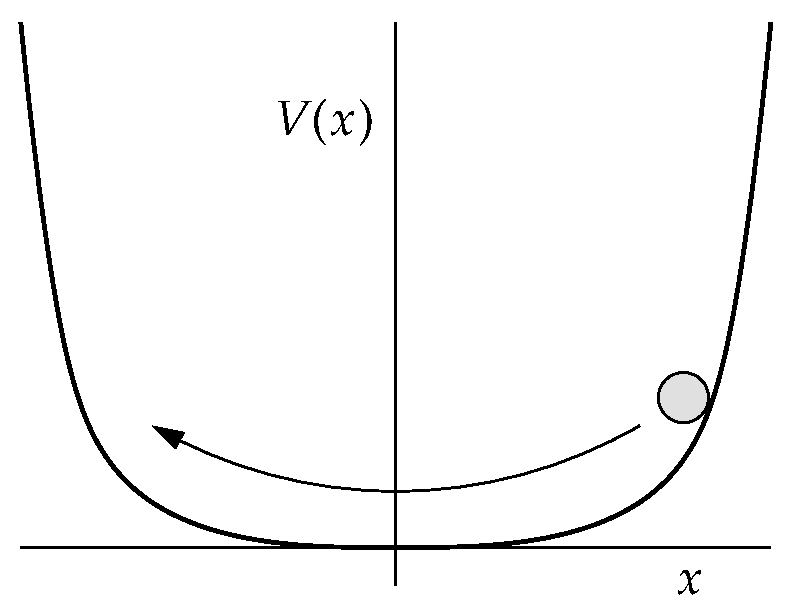
\includegraphics[width=6cm]{anharmonic.eps}
\end{center}
The harmonic oscillator corresponds to a quadratic potential $V(x) \propto
x^2$.  Any other form gives an anharmonic oscillator.  (Thus there are many
different kinds of anharmonic oscillator, depending on the exact form of
the potential.)

One way to calculate the motion of an oscillator is to write down the
equation for the conservation of energy in the system.  If the particle has
mass~$m$ and position~$x$, then the total energy is equal to the sum of the
kinetic and potential energies thus:
\begin{displaymath}
E = \half m \biggl( {\dd x\over\dd t} \biggr)^2 + V(x).
\end{displaymath}
Since the energy must be constant over time, this equation is effectively a
(nonlinear) differential equation linking $x$ and~$t$.

Let us assume that the potential~$V(x)$ is symmetric about $x=0$ and let us
set our anharmonic oscillator going with amplitude~$a$.  That is, at $t=0$
we release it from rest at position $x=a$ and it swings back towards the
origin.  Then at $t=0$ we have $\dd x/\dd t = 0$ and the equation above
reads $E = V(a)$, which gives us the total energy of the particle in terms
of the amplitude.
\begin{enumerate}\setlength{\itemsep}{0pt}
\item When the particle reaches the origin for the first time, it has gone
  through one quarter of a period of the oscillator.  By rearranging the
  equation above for $\dd x/\dd t$ and then integrating with respect to~$t$
  from 0 to $\frac14 T$, show that the period~$T$ is given by
\begin{displaymath}
T = \sqrt{8m} \int_0^a {\dd x\over\sqrt{V(a)-V(x)}}.
\end{displaymath}
\item Suppose the potential is $V(x)=x^4$ and the mass of the particle is
  $m=1$.  Write a Python function that calculates the period of the
  oscillator for given amplitude~$a$ using Gaussian quadrature with $N=20$
  points, then use your function to make a graph of the period for
  amplitudes ranging from $a=0$ to $a=2$.
\item You should find that the oscillator gets faster as the amplitude
  increases, even though the particle has further to travel for larger
  amplitude.  And you should find that the period diverges as the amplitude
  goes to zero.  How do you explain these results?
\end{enumerate}


%%% Exercise 5.11 %%%

\exercise Suppose a plane wave, such as light or a sound wave, is
blocked by an object with a straight edge, represented by the solid line at
the bottom of this figure:
\medskip
\begin{center}
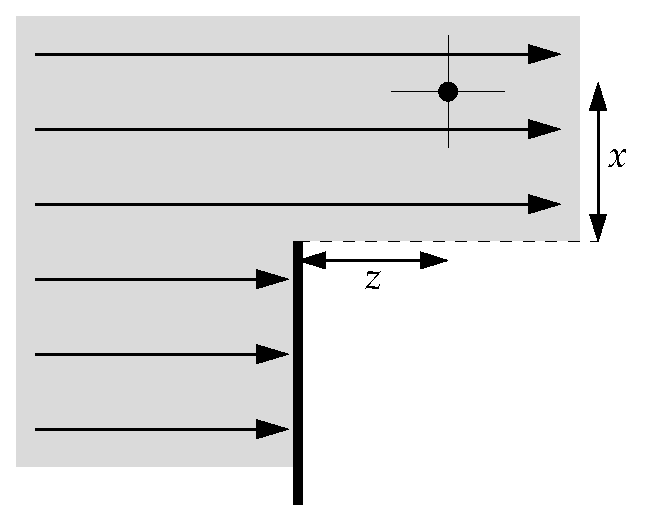
\includegraphics[width=6.5cm]{edge.eps}
\end{center}
The wave will be diffracted at the edge and the resulting intensity at the
position $(x,z)$ marked by the dot is given by near-field diffraction
theory to be
\begin{displaymath}
I = \frac{I_0}{8} \Bigl( \bigl[ 2C(u) + 1 \bigr]^2 +
                        \bigl[ 2S(u) + 1 \bigr]^2 \Bigr),
\end{displaymath}
where $I_0$ is the intensity of the wave before diffraction and
\begin{displaymath}
u = x \sqrt{2\over\lambda z}\,, \qquad
C(u) = \int_0^u \cos \half\pi t^2 \>\dd t, \qquad
S(u) = \int_0^u \sin \half\pi t^2 \>\dd t.
\end{displaymath}
Write a program to calculate $I/I_0$ and make a plot of it as a function
of~$x$ in the range $-5\,$m to~$5\,$m for the case of a sound wave with
wavelength $\lambda=1\,$m, measured $z=3\,$m past the straight edge.
Calculate the integrals using Gaussian quadrature with $N=50$ points.  You
should find significant variation in the intensity of the diffracted
sound---enough that you could easily hear the effect if sound were
diffracted, say, at the edge of a tall building.


%%% Exercise 5.12 %%%

\exercise \textbf{The Stefan--Boltzmann constant}

\exskip The Planck theory of thermal radiation tells us that in the
(angular) frequency interval $\omega$ to $\omega+\dd\omega$, a black body
of unit area radiates electromagnetically an amount of thermal energy per
second equal to $I(\omega)\>\dd\omega$, where
\begin{displaymath}
  I(\omega) = {\hbar\over4\pi^2c^2}\,{\omega^3\over(\e^{\hbar\omega/k_BT}-1)}.
\end{displaymath}
Here $\hbar$ is Planck's constant over~$2\pi$, $c$~is the speed of light,
and $k_B$ is Boltzmann's constant.
\begin{enumerate}\setlength{\itemsep}{0pt}
\item Show that the total energy per unit area radiated by a black body is
\begin{displaymath}
W = {k_B^4 T^4\over4\pi^2c^2\hbar^3} \int_0^\infty {x^3\over\e^x-1}\>\dd x.
\end{displaymath}
\item Write a program to evaluate the integral in this expression.  Explain
  what method you used, and how accurate you think your answer is.
\item Even before Planck gave his theory of thermal radiation around the
  turn of the 20th century, it was known that the total energy~$W$ given
  off by a black body per unit area per second followed Stefan's
  law: $W = \sigma T^4$, where $\sigma$ is the Stefan--Boltzmann constant.
  Use your value for the integral above to compute a value for the
  Stefan--Boltzmann constant (in SI units) to three significant figures.
  Check your result against the known value, which you can find in books or
  on-line.  You should get good agreement.
\end{enumerate}


%%% Exercise 5.13 %%%

\exercise \textbf{Quantum uncertainty in the harmonic oscillator}

\exskip In units where all the constants are~1, the wavefunction of the
$n$th energy level of the one-dimensional quantum harmonic
oscillator---i.e.,~a spinless point particle in a quadratic potential
well---is given by
\begin{displaymath}
\psi_n(x) = {1\over\sqrt{2^n n!\sqrt{\pi}}}\, \e^{-x^2/2}\,H_n(x),
\end{displaymath}
for $n=0\ldots\infty$, where $H_n(x)$ is the $n$th Hermite
polynomial.  Hermite polynomials satisfy a relation somewhat similar to
that for the Fibonacci numbers, although more complex:
\begin{displaymath}
H_{n+1}(x) = 2xH_n(x) - 2nH_{n-1}(x).
\end{displaymath}
The first two Hermite polynomials are $H_0(x)=1$ and $H_1(x)=2x$.

\begin{enumerate}\setlength{\itemsep}{0pt}
\item Write a user-defined function~\verb|H(n,x)| that calculates $H_n(x)$
  for given~$x$ and any integer $n\ge0$.  Use your function to make a plot
  that shows the harmonic oscillator wavefunctions for $n=0$, 1, 2, and~3,
  all on the same graph, in the range $x=-4$ to $x=4$.  Hint: There is a
  function \verb|factorial| in the \verb|math| package that
  calculates the factorial of an integer.
\item Make a separate plot of the wavefunction for $n=30$ from $x=-10$ to
  $x=10$.  Hint: If your program takes too long to run in this case, then
  you're doing the calculation wrong---the program should take only a
  second or so to run.
\item The quantum uncertainty of a particle in the $n$th level of a quantum
  harmonic oscillator can be quantified by its root-mean-square position
  $\sqrt{\av{x^2}}$, where
\begin{displaymath}
\av{x^2} = \int_{-\infty}^\infty x^2 |\psi_n(x)|^2 \>\dd x.
\end{displaymath}
Write a program that evaluates this integral using Gaussian quadrature on
100 points and then calculates the uncertainty (i.e.,~the root-mean-square
position of the particle) for a given value of~$n$.  Use your program to
calculate the uncertainty for $n=5$.  You should get an answer in the
vicinity of~$\sqrt{\av{x^2}}=2.3$.
\end{enumerate}


%%% Exercise 5.14 %%%

\exercise \textbf{Gravitational pull of a uniform sheet}

\exskip A uniform square sheet of metal is floating motionless in space:
\begin{center}
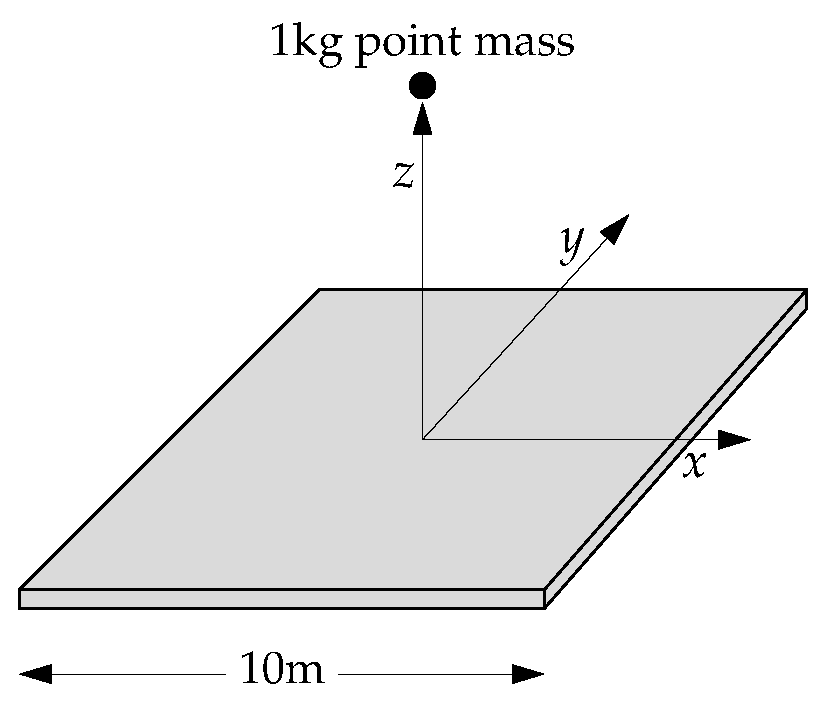
\includegraphics[width=6.5cm]{plate.eps}
\end{center}
The sheet is $10\,$m on a side and of negligible thickness, and it has a
mass of 10 metric tonnes.
\begin{enumerate}\setlength{\itemsep}{0pt}
\item Consider the gravitational force due to the plate felt by a point
  mass of $1\,$kg a distance~$z$ from the center of the square, in the
  direction perpendicular to the sheet, as shown above.  Show that the
  component of the force along the $z$-axis is
\begin{displaymath}
F_z = G\sigma z \iint_{-L/2}^{L/2} {\dd x\,\dd y\over(x^2+y^2+z^2)^{3/2}}\,,
\end{displaymath}
where
$G=6.674\times10^{-11}\,\mathrm{m}^3\,\mathrm{kg}^{-1}\,\mathrm{s}^{-2}$ is
Newton's gravitational constant and $\sigma$ is the mass per unit area of
the sheet.
\item Write a program to calculate and plot the force as a function of $z$
  from $z=0$ to $z=10\,$m.  For the double integral use (double) Gaussian
  quadrature, as in Eq.~(5.82), with 100 sample points along each axis.
\item You should see a smooth curve, except at very small values of~$z$,
  where the force should drop off suddenly to zero.  This drop is not a
  real effect, but an artifact of the way we have done the calculation.
  Explain briefly where this artifact comes from and suggest a strategy to
  remove it, or at least to decrease its size.
\end{enumerate}
This calculation can thought of as a model for the gravitational pull of a
galaxy.  Most of the mass in a spiral galaxy (such as our own Milky Way)
lies in a thin plane or disk passing through the galactic center, and the
gravitational pull exerted by that plane on bodies outside the galaxy can
be calculated by just the methods we have employed here.


%%% Exercise 5.15 %%%

\exercise Create a user-defined function~\verb|f(x)| that returns the value
$1 + \half \tanh2x$, then use a central difference to calculate the
derivative of the function in the range $-2\le x\le2$.  Calculate an
analytic formula for the derivative and make a graph with your numerical
result and the analytic answer on the same plot.  It may help to plot the
exact answer as lines and the numerical one as dots.  (Hint: In Python the
tanh function is found in the \verb|math| package, and it's called simply
\verb|tanh|.)


%%% Exercise 5.16 %%%

\exercise Even when we can find the value of $f(x)$ for any value of~$x$
the forward difference can still be more accurate than the central
difference for sufficiently large~$h$.  For what values of~$h$ will the
approximation error on the forward difference of Eq.~(5.87) be smaller than
on the central difference of Eq.~(5.95)?


%%% Exercise 5.17 %%%

\exercise \textbf{The gamma function}

\exskip A commonly occurring function in physics calculations is the
gamma function~$\Gamma(a)$, which is defined by the integral
\begin{displaymath}
\Gamma(a) = \int_0^\infty x^{a-1} \e^{-x} \>\dd x.
\end{displaymath}
There is no closed-form expression for the gamma function, but one can
calculate its value for given~$a$ by performing the integral above
numerically.  You have to be careful how you do it, however, if you wish to
get an accurate answer.
\begin{enumerate}\setlength{\itemsep}{0pt}
\item Write a program to make a graph of the value of the integrand
  $x^{a-1} \e^{-x}$ as a function of~$x$ from $x=0$ to $x=5$, with three
  separate curves for $a=2$, 3, and~4, all on the same axes.  You should
  find that the integrand starts at zero, rises to a maximum, and then
  decays again for each curve.
\item Show analytically that the maximum falls at $x=a-1$.
\item Most of the area under the integrand falls near the maximum, so to
  get an accurate value of the gamma function we need to do a good job of
  this part of the integral. We can change the integral from 0 to $\infty$
  to one over a finite range from 0 to 1 using the change of variables in
  Eq.~(5.67), but this tends to squash the peak towards the edge of the
  $[0,1]$ range and does a poor job of evaluating the integral accurately.
  We can do a better job by making a different change of variables that
  puts the peak in the middle of the integration range, around~$\half$.  We
  will use the change of variables given in Eq.~(5.69), which we repeat
  here for convenience:
\begin{displaymath}
z = {x\over c+x}.
\end{displaymath}
For what value of $x$ does this change of variables give~$z=\half$?  Hence
what is the appropriate choice of the parameter~$c$ that puts the peak of
the integrand for the gamma function at $z=\half$?
\item Before we can calculate the gamma function, there is another detail
  we need to attend to.  The integrand $x^{a-1} \e^{-x}$ can be difficult
  to evaluate because the factor~$x^{a-1}$ can become very large and the
  factor $\e^{-x}$ very small, causing numerical overflow or underflow, or
  both, for some values of~$x$.  Write $x^{a-1}=\e^{(a-1)\ln x}$ to derive
  an alternative expression for the integrand that does not suffer from
  these problems (or at least not so much).  Explain why your new
  expression is better than the old one.
\item Now, using the change of variables above and the value of~$c$ you
  have chosen, write a user-defined function \verb|gamma(a)| to calculate
  the gamma function for arbitrary argument~$a$.  Use whatever integration
  method you feel is appropriate.  Test your function by using it to
  calculate and print the value of~$\Gamma(\frac32)$, which is known to be
  equal to $\frac12\sqrt{\pi}\simeq0.886$.
\item For integer values of $a$ it can be shown that $\Gamma(a)$ is equal
  to the factorial of $a-1$.  Use your Python function to calculate
  $\Gamma(3)$, $\Gamma(6)$, and $\Gamma(10)$.  You should get answers
  closely equal to $2!=2$, $5!=120$, and $9!=362\,880$.
\end{enumerate}


%%% Exercise 5.18 %%%

\exercise Rearranging Eq.~(5.19) into a slightly more conventional form, we
have:
\begin{displaymath}
\int_a^b f(x)\>\dd x
  = h \biggl[ \half f(a) + \half f(b) + \sum_{k=1}^{N-1} f(a+kh)
            \biggr] + \tfrac{1}{12} h^2 \bigl[ f'(a) - f'(b) \bigr] +
            \Ord(h^4).
\end{displaymath}
This result gives a value for the integral on the left which has an error
of order~$h^4$---a factor of $h^2$ better than the error on the trapezoidal
rule and as good as Simpson's rule.  We can use this formula as a new rule
for evaluating integrals, distinct from any of the others we have seen in
this chapter.  We might call it the ``Euler--Maclaurin rule.''
\begin{enumerate}\setlength{\itemsep}{0pt}
\item Write a program to calculate the value of the integral $\int_0^2
  (x^4-2x+1) \>\dd x$ using this formula.  (This is the same integral that
  we studied in Example~5.1, whose true value is~4.4.)  The order-$h$ term
  in the formula is just the ordinary trapezoidal rule; the $h^2$ term
  involves the derivatives $f'(a)$ and $f'(b)$, which you should evaluate
  using central differences, centered on $a$ and $b$ respectively.  Note
  that the size of the interval you use for calculating the central
  differences does not have to equal the value of $h$ used in the
  trapezoidal rule part of the calculation.  An interval of about $10^{-5}$
  gives good values for the central differences.

  Use your program to evaluate the integral with $N=10$ slices and compare
  the accuracy of the result with that obtained from the trapezoidal rule
  alone with the same number of slices.
\item Good though it is, this integration method is not much used in
  practice.  Suggest a reason why not.
\end{enumerate}


%%% Exercise 5.19 %%%

\exercise \textbf{Diffraction gratings}

\exskip Light with wavelength~$\lambda$ is incident on a diffraction
grating of total width~$w$, gets diffracted, is focused with a lens of
focal length~$f$, and falls on a screen:
\begin{center}
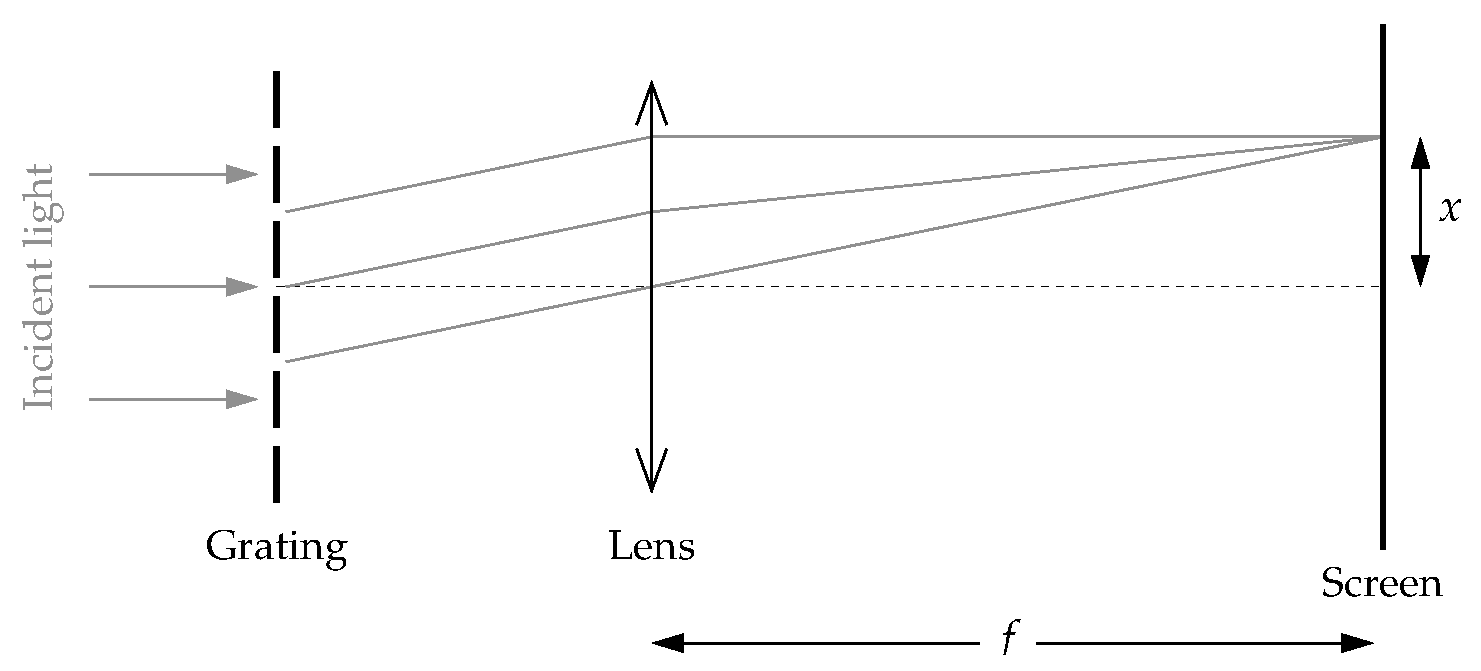
\includegraphics[width=13cm]{diffraction.eps}
\end{center}
\medskip
Theory tells us that the intensity of the diffraction pattern on the
screen, a distance~$x$ from the central axis of the system, is given by
\begin{displaymath}
I(x) = \biggl| \int_{-w/2}^{w/2} \sqrt{q(u)}\>
               \e^{\ii 2\pi xu/\lambda f} \>\dd u \biggr|^2,
\end{displaymath}
where $q(u)$ is the intensity transmission function of the diffraction
grating at a distance~$u$ from the central axis, i.e.,~the fraction of the
incident light that the grating lets through.
\begin{enumerate}\setlength{\itemsep}{0pt}
\item Consider a grating with transmission function $q(u) = \sin^2 \alpha
  u$.  What is the separation of the ``slits'' in this grating, expressed
  in terms of~$\alpha$?
\item Write a Python function \verb|q(u)| that returns the transmission
  function $q(u) = \sin^2 \alpha u$ as above at position~$u$ for a grating
  whose slits have separation $20\,\mu$m.
\item Use your function in a program to calculate and graph the intensity
  of the diffraction pattern produced by such a grating having ten slits in
  total, if the incident light has wavelength $\lambda=500\,$nm.  Assume
  the lens has a focal length of 1~meter and the screen is $10\,$cm wide.
  You can use whatever method you think appropriate for doing the integral.
  Once you've made your choice you'll also need to decide the number of
  sample points you'll use.  What criteria play into this decision?

  Notice that the integrand in the equation for~$I(x)$ is complex, so you
  will have to use complex variables in your program.  As mentioned in
  Section~2.2.5, there is a version of the \verb|math| package for use with
  complex variables called \verb|cmath|.  In particular you may find the
  \verb|exp| function from \verb|cmath| useful because it can calculate the
  exponentials of complex arguments.
\item Create a visualization of how the diffraction pattern would look on
  the screen using a density plot (see Section~3.3).  Your plot should look
  something like this: \medskip
\begin{center}

\includegraphics[width=12cm]{pattern.eps}
\end{center}
\smallskip
\item Modify your program further to make pictures of the diffraction
  patterns produced by gratings with the following profiles:
{\renewcommand{\labelenumii}{\roman{enumii})\ }
\begin{enumerate}\setlength{\itemsep}{0pt}
\item A transmission profile that obeys $q(u) = \sin^2\alpha u\,
  \sin^2\beta u$, with $\alpha$ as before and the same total grating
  width~$w$, and $\beta=\half\alpha$.
\item Two ``square'' slits, meaning slits with 100\% transmission through
  the slit and 0\% transmission everywhere else.  Calculate the diffraction
  pattern for non-identical slits, one $10\,\mu$m wide and the other
  $20\,\mu$m wide, with a $60\,\mu$m gap between the two.
\end{enumerate}}
\end{enumerate}


%%% Exercise 5.20 %%%

\exercise \textbf{A more advanced adaptive method for the trapezoidal
  rule}

\exskip In Section~5.3 we studied an adaptive version of the trapezoidal
rule in which the number of steps is increased---and the width~$h$ of the
slices correspondingly decreased---until the calculation gives a value for
the integral accurate to some desired level.  Although this method
varies~$h$, it still calculates the integral at any individual stage of the
process using slices of equal width throughout the domain of integration.
In this exercise we look at a more sophisticated form of the trapezoidal
rule that uses different step sizes in different parts of the domain, which
can be useful particularly for poorly behaved functions that vary rapidly
in certain regions but not others.  Remarkably, this method is not much
more complicated to program than the ones we've already seen, if one knows
the right tricks.  Here's how the method works.

  Suppose we wish to evaluate the integral $I = \int_a^b f(x) \>\dd x$ and
  we want an error of no more than~$\epsilon$ on our answer.  To put that
  another way, if we divide up the integral into slices of width~$h$ then
  we require an accuracy per slice~of
\begin{displaymath}
h\,{\epsilon\over b-a} = h\delta,
\end{displaymath}
where $\delta = \epsilon/(b-a)$ is the target accuracy per unit interval.

We start by evaluating the integral using the trapezoidal rule with just a
single slice of width $h_1=b-a$.  Let us call the estimate of the integral
from this calculation~$I_1$.  Usually $I_1$ will not be very accurate, but
let us ignore that for the moment.  Next we make a second estimate~$I_2$ of
the integral, again using the trapezoidal rule but now with two slices of
width $h_2=\half h_1$ each.  Equation~(5.28) tells us that the error on
this second estimate is $\frac13(I_2-I_1)$ to leading order.  If this error
is smaller than the desired accuracy~$h_2\delta$ then our calculation is
complete and we need go no further.  $I_2$~is a good enough estimate of the
integral.

Most likely, however, this will not be the case; the accuracy will not be
good enough.  If so, then we divide the integration interval into two equal
parts of size $\half (b-a)$ each, and we repeat the process above in each
part separately, calculating estimates $I_1$ and $I_2$ using one and two
slices respectively, estimating the error, and checking to see if it is
less than $h_2\delta$ (with the new value of $h_2$ now).

We keep on repeating this process, dividing each slice in half and in half
again, as many times as necessary to achieve the desired accuracy in every
slice.  Different slices may be divided different numbers of times, and
hence we may end up with different sized slices in different parts of the
integration domain.  The method automatically uses whatever size and number
of slices is appropriate in each region.
\begin{enumerate}\setlength{\itemsep}{0pt}
\item Write a program using this method to calculate the integral
\begin{displaymath}
I = \int_0^{10} {\sin^2 x\over x^2} \>\dd x,
\end{displaymath}
to an accuracy of $\epsilon=10^{-4}$.  Start by writing a function to
calculate the integrand $f(x) = (\sin^2 x)/x^2$.  Note that the limiting
value of the integrand at $x=0$ is~1.  You'll probably have to include this
point as a special case in your function using an if statement.

The best way to perform the integration itself is to make use of the
technique of recursion, the ability of a Python function to call itself.
(If you're not familiar with recursion, you may like to look at
Exercise~2.13 on page~83 before doing this exercise.)  Write a function
\verb|step(x1,x2,f1,f2)| that takes as arguments the beginning and end
points~$x_1,x_2$ of a slice and the values $f(x_1), f(x_2)$ of the
integrand at those two points, and returns the value of the integral from
$x_1$ to~$x_2$.  This function should evaluate the two estimates~$I_1$
and~$I_2$ of the integral from $x_1$ to~$x_2$, calculated with one and two
slices respectively, and the error $\frac13(I_2-I_1)$.  If this error meets
the target value, which is $\half(x_2-x_1)\delta$, then the calculation is
complete and the function simply returns the value~$I_2$.  If the error
fails to meet the target, then the function calls itself, twice, to
evaluate the integral separately on the first and second halves of the
interval and returns the sum of the two results.  (And then \emph{those}
functions can call themselves, and so forth, subdividing the integral as
many times as necessary to reach the required accuracy.)

Hint: As icing on the cake, when the error target is met and the function
returns a value for the integral in the current slice, it can, in fact,
return a slightly better value than the estimate~$I_2$.  Since you will
already have calculated the value of the integrand~$f(x)$ at $x_1$, $x_2$,
and the midpoint $x_m=\half(x_1+x_2)$ in order to evaluate~$I_2$, you can
use those results to compute the improved Simpson's rule estimate,
Eq.~(5.7), for this slice.  You just return the value $\frac16
h[f(x_1)+4f(x_m)+f(x_2)]$ instead of the trapezoidal rule estimate $\frac14
h[f(x_1)+2f(x_m)+f(x_2)]$ (where $h=x_2-x_1$).  This involves very little
extra work, but gives a value that is more accurate by two orders in~$h$.
(Technically, this is an example of the method of ``local extrapolation,''
although it's perhaps not obvious what we're extrapolating in this case.
We'll discuss local extrapolation again when we study adaptive methods for
the solution of differential equations in Section~8.4.)
\item Why does the function \verb|step(x1,x2,f1,f2)| take not only the
  positions $x_1$ and~$x_2$ as arguments, but also the values $f(x_1)$
  and~$f(x_2)$?  Since we know the function~$f(x)$, we could just calculate
  these values from $x_1$ and~$x_2$.  Nonetheless, it is a smart move to
  include the values of $f(x_1)$ and~$f(x_2)$ as arguments to the function.
  Why?
\item Modify your program to make a plot of the integrand with dots added
  showing where the ends of each integration slice lie.  You should see
  larger slices in portions of the integrand that follow reasonably
  straight lines (because the trapezoidal rule gives an accurate value for
  straight-line integrands) and smaller slices in portions with more
  curvature.
\end{enumerate}


%%% Exercise 5.21 %%%

\exercise \textbf{Electric field of a charge distribution}

\exskip Suppose we have a distribution of charges and we want to calculate
the resulting electric field.  One way to do this is to first calculate the
electric potential~$\phi$ and then take its gradient.  For a point
charge~$q$ at the origin, the electric potential at a distance~$r$ from the
origin is $\phi=q/4\pi\epsilon_0 r$ and the electric field is $\vec{E} =
-\nabla\phi$.
\begin{enumerate}\setlength{\itemsep}{0pt}
\item You have two charges, of $\pm1\,$C, $10\,$cm apart.  Calculate the
  resulting electric potential on a $1\,\textrm{m}\times1\,\textrm{m}$
  square plane surrounding the charges and passing through them.  Calculate
  the potential at $1\,$cm spaced points in a grid and make a
  visualization on the screen of the potential using a density plot.
\item Now calculate the partial derivatives of the potential with respect
  to $x$ and $y$ and hence find the electric field in the $xy$ plane.  Make
  a visualization of the field also.  This is a little trickier than
  visualizing the potential, because the electric field has both magnitude
  and direction.  One way to do it might be to make two density plots, one
  for the magnitude, and one for the direction, the latter using the
  ``\verb|hsv|'' color scheme in \verb|pylab|, which is a rainbow scheme
  that passes through all the colors but starts and ends with the same
  shade of red, which makes it suitable for representing things like
  directions or angles that go around the full circle and end up where they
  started.  A more sophisticated visualization might use the arrow
  object from the \verb|visual| package, drawing a grid of arrows with
  direction and length chosen to represent the field.
\item Now suppose you have a continuous distribution of charge over an
  $L\times L$ square.  The charge density in Cm$^{-2}$ is
\begin{displaymath}
\sigma(x,y) = q_0 \sin {2\pi x\over L} \sin{2\pi y\over L}.
\end{displaymath}
Calculate and visualize the resulting electric field at $1\,$cm-spaced
points in 1~square meter of the $xy$ plane for the case where $L=10\,$cm,
the charge distribution is centered in the middle of the visualized area,
and $q_0=100\,\textrm{Cm}^{-2}$.  You will have to perform a double
integral over $x$ and~$y$, then differentiate the potential with respect to
position to get the electric field.  Choose whatever integration method
seems appropriate for the integrals.
\end{enumerate}


%%% Exercise 5.22 %%%

\exercise \textbf{Differentiating by integrating}

\exskip If you are familiar with the calculus of complex variables, you may
find the following technique useful and interesting.

Suppose we have a function~$f(z)$ whose value we know not only on the real
line but also for complex values of its argument.  Then we can calculate
derivatives of that function at any point~$z_0$ by performing a contour
integral, using the Cauchy derivative formula:
\begin{displaymath}
\biggl( {\dd^m\!f\over\dd z^m} \biggr)_{z=z_0}
  = {m!\over2\pi\ii} \oint {f(z)\over(z-z_0)^{m+1}} \>\dd z,
\end{displaymath}
where the integral is performed counterclockwise around any contour in the
complex plane that surrounds the point~$z_0$ but contains no poles
in~$f(z)$.  Since numerical integration is significantly easier and more
accurate than numerical differentiation, this formula provides us with a
method for calculating derivatives---and especially multiple
derivatives---accurately by turning them into integrals.

Suppose, for example, that we want to calculate derivatives of $f(z)$ at
$z=0$.  Let us apply the Cauchy formula above using the trapezoidal rule to
calculate the integral along a circular contour centered on the origin with
radius~1.  The trapezoidal rule will be slightly different from the version
we are used to because the value of the interval~$h$ is now a complex
number, and moreover is not constant from one slice of the integral to the
next---it stays constant in modulus, but its argument changes from one
slice to another.

We will divide our contour integral into $N$ slices with sample
points~$z_k$ distributed uniformly around the circular contour at the
positions $z_k = \e^{\ii 2\pi k/N}$ for $k=0\ldots N$.  Then the distance
between consecutive sample points is
\begin{displaymath}
h_k = z_{k+1} - z_k = \e^{\ii 2\pi(k+1)/N} - \e^{\ii 2\pi k/N},
\end{displaymath}
and, introducing the shorthand $g(z)=f(z)/z^{m+1}$ for the integrand, the
trapezoidal rule approximation to the integral is
\begin{align*}
\oint g(z) \>\dd z
  &\simeq \sum_{k=0}^{N-1} \half \bigl[ g(z_{k+1}) + g(z_k) \bigr]
          \bigl[ \e^{\ii 2\pi(k+1)/N} - \e^{\ii 2\pi k/N} \bigr] \\
  &= \half \biggl[ \sum_{k=0}^{N-1} g(z_{k+1})\,\e^{\ii 2\pi(k+1)/N}
                   - \sum_{k=0}^{N-1} g(z_k)\,\e^{\ii 2\pi k/N} \\
  &\hspace{4em}{}  - \sum_{k=0}^{N-1} g(z_{k+1})\,\e^{\ii 2\pi k/N}
                   + \sum_{k=0}^{N-1} g(z_k)\,\e^{\ii 2\pi(k+1)/N}
           \biggr].
\end{align*}
Noting that $z_N=z_0$, the first two sums inside the brackets cancel each
other in their entirety, and the remaining two sums are equal except for
trivial phase factors, so the entire expression simplifies to
\begin{align*}
\oint g(z) \>\dd z
  &\simeq \half \bigl[ \e^{\ii2\pi/N}-\e^{-\ii2\pi/N} \bigr]
          \sum_{k=0}^{N-1} g(z_k)\,\e^{\ii2\pi k/N} \\
  &\simeq {2\pi\ii\over N} \sum_{k=0}^{N-1} f(z_k)\,\e^{-\ii2\pi km/N},
\end{align*}
where we have used the definition of $g(z)$ again.  Combining this result
with the Cauchy formula, we then have
\begin{displaymath}
\biggl( {\dd^m\!f\over\dd z^m} \biggr)_{z=0}
  \simeq {m!\over N} \sum_{k=0}^{N-1} f(z_k)\,\e^{-\ii2\pi km/N}.
\end{displaymath}

Write a program to calculate the first twenty derivatives of $f(z)=\e^{2z}$
at $z=0$ using this formula with $N=10000$.  You will need to use the
version of the \verb|exp| function from the \verb|cmath| package, which can
handle complex arguments.  You may also find the function \verb|factorial|
from the \verb|math| package useful; it calculates factorials of integer
arguments.

The correct value for the $m$th derivative in this case is easily shown to
be~$2^m$, so it should be straightforward to tell if your program is
working---the results should be powers of two, 2, 4, 8, 16, 32, etc.  You
should find that it is possible to get reasonably accurate results for all
twenty derivatives rapidly using this technique.  If you use standard
difference formulas for the derivatives, on the other hand, you will find
that you can calculate only the first three or four derivatives accurately
before the numerical errors become so large that the results are useless.
In this case, therefore, the Cauchy formula gives the better results.

The sum $\sum_k f(z_k)\,\e^{\ii2\pi km/N}$ that appears in the formula
above is known as the \defn{discrete Fourier transform} of the complex
samples~$f(z_k)$.  There exists an elegant technique for evaluating the
Fourier transform for many values of~$m$ simultaneously, known as the
\defn{fast Fourier transform}, which could be useful in cases where the
direct evaluation of the formula is slow.  We will study the fast Fourier
transform in detail in Chapter~7.



%%% Exercise 5.23 %%%

\exercise \textbf{Image processing and the STM}

\exskip When light strikes a surface, the amount falling per unit area
depends not only on the intensity of the light, but also on the angle of
incidence.  If the light makes an angle~$\theta$ to the normal, it only
``sees'' $\cos\theta$ of area per unit of actual area on the surface:
\bigskip
\begin{center}
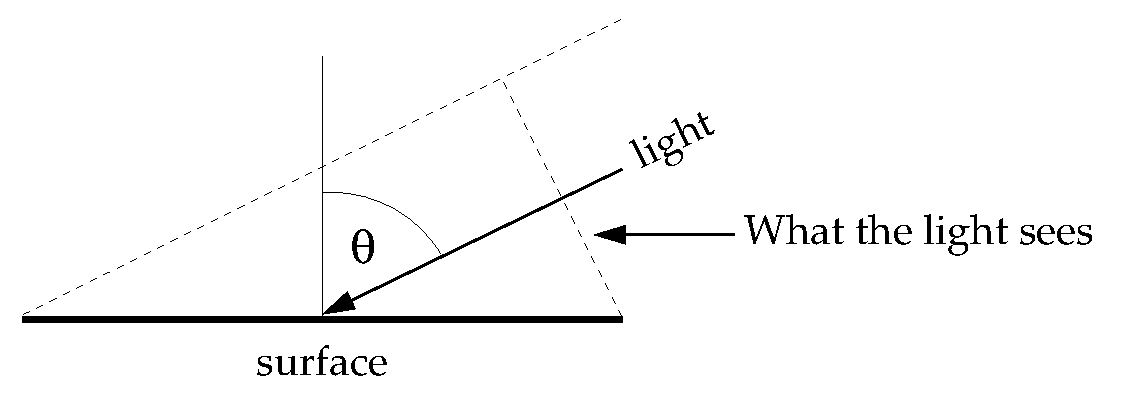
\includegraphics[width=10cm]{light.eps}
\end{center}
\medskip
So the intensity of illumination is $a\cos\theta$, if $a$ is the raw
intensity of the light.  This simple physical law is a central element of
3D computer graphics.  It allows us to calculate how light falls on
three-dimensional objects and hence how they will look when illuminated
from various angles.

Suppose, for instance, that we are looking down on the Earth from above and
we see mountains.  We know the height of the mountains $w(x,y)$ as a
function of position in the plane, so the equation for the Earth's
surface is simply $z=w(x,y)$, or equivalently $w(x,y)-z=0$, and the normal
vector~$\vec{v}$ to the surface is given by the gradient of $w(x,y)-z$
thus:
\begin{displaymath}
\vec{v} =
\nabla [w(x,y)-z] = \begin{pmatrix}
                  \partial/\partial x \\
                  \partial/\partial y \\
                  \partial/\partial z
                \end{pmatrix}
                [w(x,y)-z]
              = \begin{pmatrix}
                  \partial w/\partial x \\
                  \partial w/\partial y \\
                  -1
                \end{pmatrix}.
\end{displaymath}
Now suppose we have light coming in represented by a vector~$\vec{a}$ with
magnitude equal to the intensity of the light.  Then the dot product of the
vectors $\vec{a}$ and~$\vec{v}$ is
\begin{displaymath}
\vec{a}\cdot\vec{v} = |\vec{a}|\,|\vec{v}|\cos\theta,
\end{displaymath}
where $\theta$ is the angle between the vectors.  Thus the intensity of
illumination of the surface of the mountains is
\begin{displaymath}
I = |\vec{a}| \cos\theta = {\vec{a}\cdot\vec{v}\over|\vec{v}|}
  = {a_x (\partial w/\partial x)
   + a_y (\partial w/\partial y) - a_z\over
     \sqrt{(\partial w/\partial x)^2 + (\partial w/\partial y)^2 + 1}}.
\end{displaymath}
Let's take a simple case where the light is shining horizontally with unit
intensity, along a line an angle~$\phi$ counter-clockwise from the
east-west axis, so that $\vec{a}=(\cos\phi,\sin\phi,0)$.  Then our
intensity of illumination simplifies to
\begin{displaymath}
I = {\cos\phi\,(\partial w/\partial x) + \sin\phi\,(\partial w/\partial y)\over
     \sqrt{(\partial w/\partial x)^2 + (\partial w/\partial y)^2 + 1}}.
\end{displaymath}
If we can calculate the derivatives of the height~$w(x,y)$ and we
know~$\phi$ we can calculate the intensity at any point.

\begin{enumerate}\setlength{\itemsep}{0pt}
\item In the on-line resources you'll find a file called
  \verb|altitude.txt|, which contains the altitude~$w(x,y)$ in meters above
  sea level (or depth below sea level) of the surface of the Earth,
  measured on a grid of points~$(x,y)$.  Write a program that reads this
  file and stores the data in an array.  Then calculate the derivatives
  $\partial w/\partial x$ and $\partial w/\partial y$ at each grid point.
  Explain what method you used to calculate them and why.  (Hint: You'll
  probably have to use more than one method to get every grid point,
  because awkward things happen at the edges of the grid.)  To calculate
  the derivatives you'll need to know the value of~$h$, the distance in
  meters between grid points, which is about $30\,000\,$m in this case.
  (It's actually not precisely constant because we are representing the
  spherical Earth on a flat map, but $h=30\,000\,$m will give reasonable
  results.)
\item Now, using your values for the derivatives, calculate the intensity
  for each grid point, with $\phi=45^\circ$, and make a density plot of the
  resulting values in which the brightness of each dot depends on the
  corresponding intensity value.  If you get it working right, the plot
  should look like a relief map of the world---you should be able to see
  the continents and mountain ranges in 3D.  (Common problems include a map
  that is upside-down or sideways, or a relief map that is ``inside-out,''
  meaning the high regions look low and \textit{vice versa}.  Work with the
  details of your program until you get a map that looks right to you.)
\item There is another file in the on-line resources called \verb|stm.txt|,
  which contains a grid of values from scanning tunneling microscope
  measurements of the (111) surface of silicon.  A scanning
  tunneling microscope (STM) is a device that measures the shape of
  surfaces at the atomic level by tracking a sharp tip over the surface and
  measuring quantum tunneling current as a function of position.  The end
  result is a grid of values that represent the height of the surface as a
  function of position and the data in the file \verb|stm.txt| contain just
  such a grid of values.  Modify the program you just wrote to visualize
  the STM data and hence create a 3D picture of what the silicon
  surface looks like.  The value of~$h$ for the derivatives in this case is
  around $h=2.5$ (in arbitrary units).
\end{enumerate}

\end{exercises}

\end{document}
